% Lossless views of the accepted 1800x1120 kernel image (72 dpi).
% The original image also supplies the separate blue-channel enlargement.
\begin{minipage}[t]{0.31\linewidth}
    \centering
    {\sffamily\small Canal rojo\par}\smallskip
    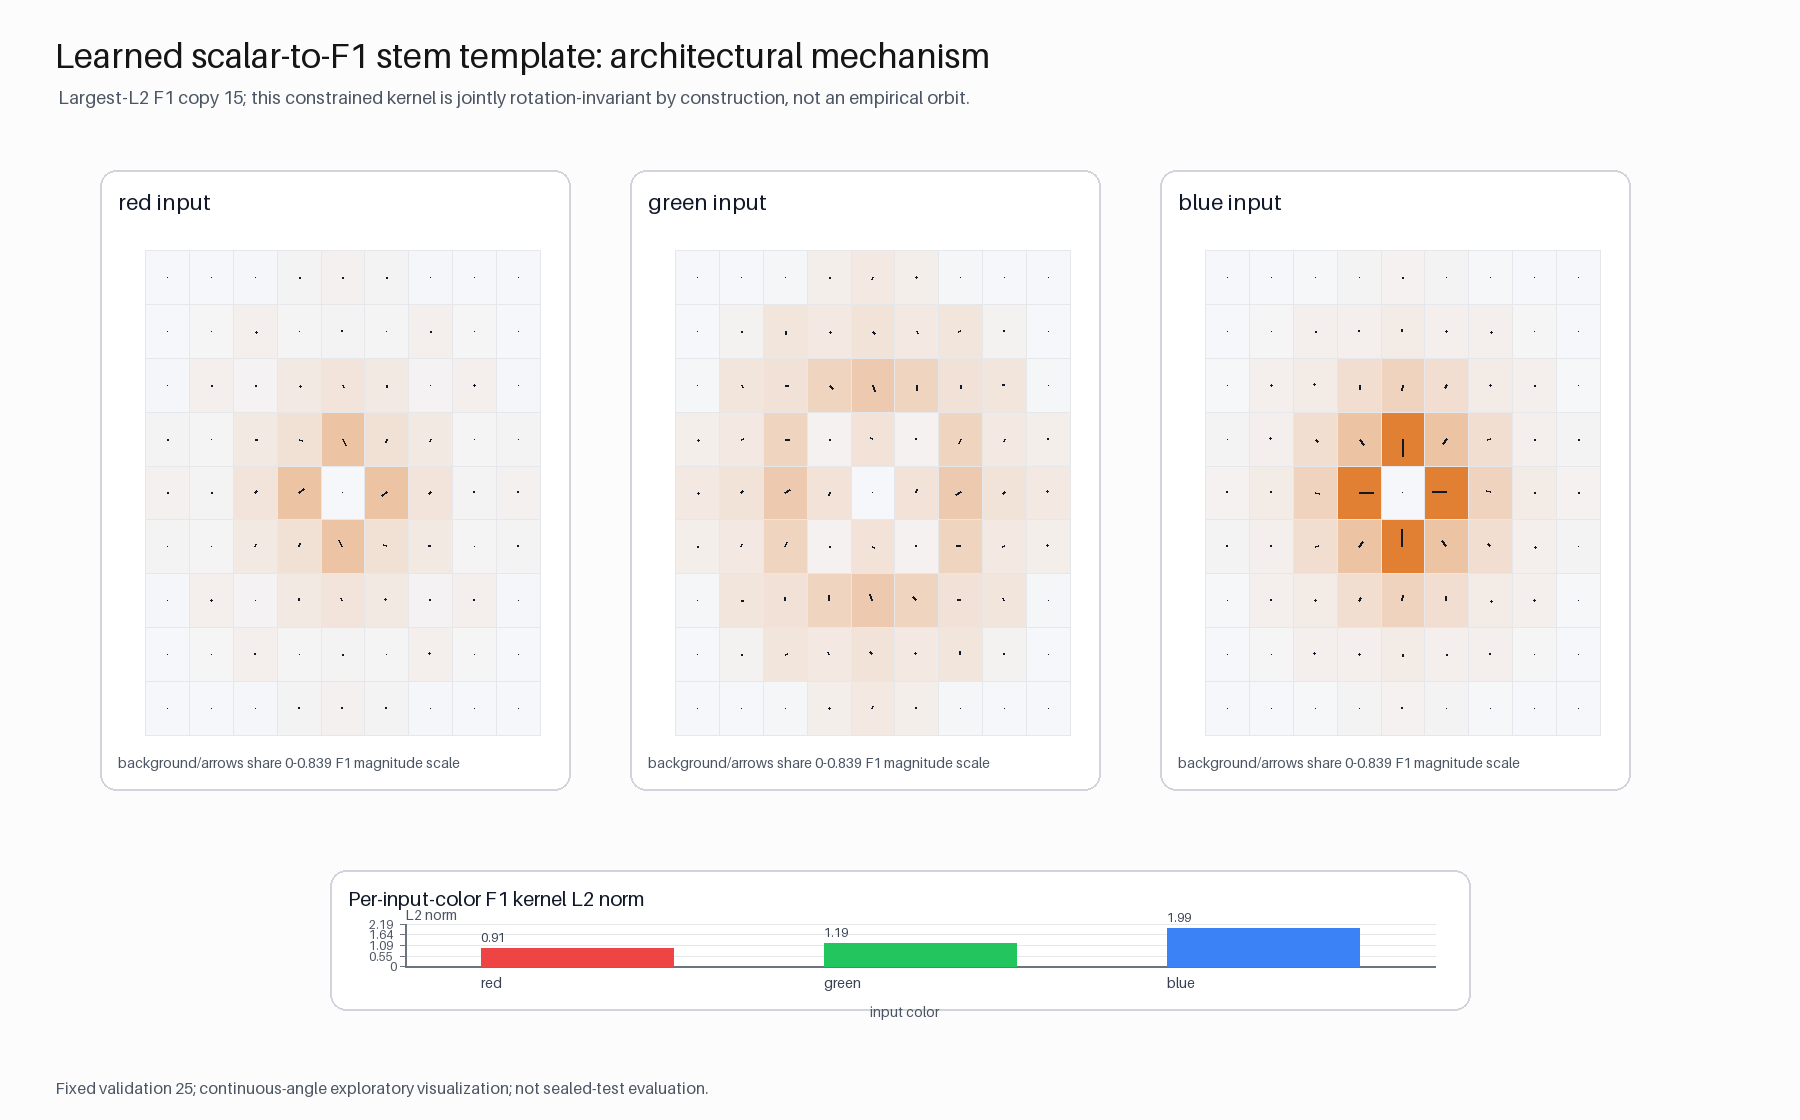
\includegraphics[width=\linewidth,trim=140 378 1255 245,clip]
        {so2_stem_kernel_f1.png}
\end{minipage}\hfill
\begin{minipage}[t]{0.31\linewidth}
    \centering
    {\sffamily\small Canal verde\par}\smallskip
    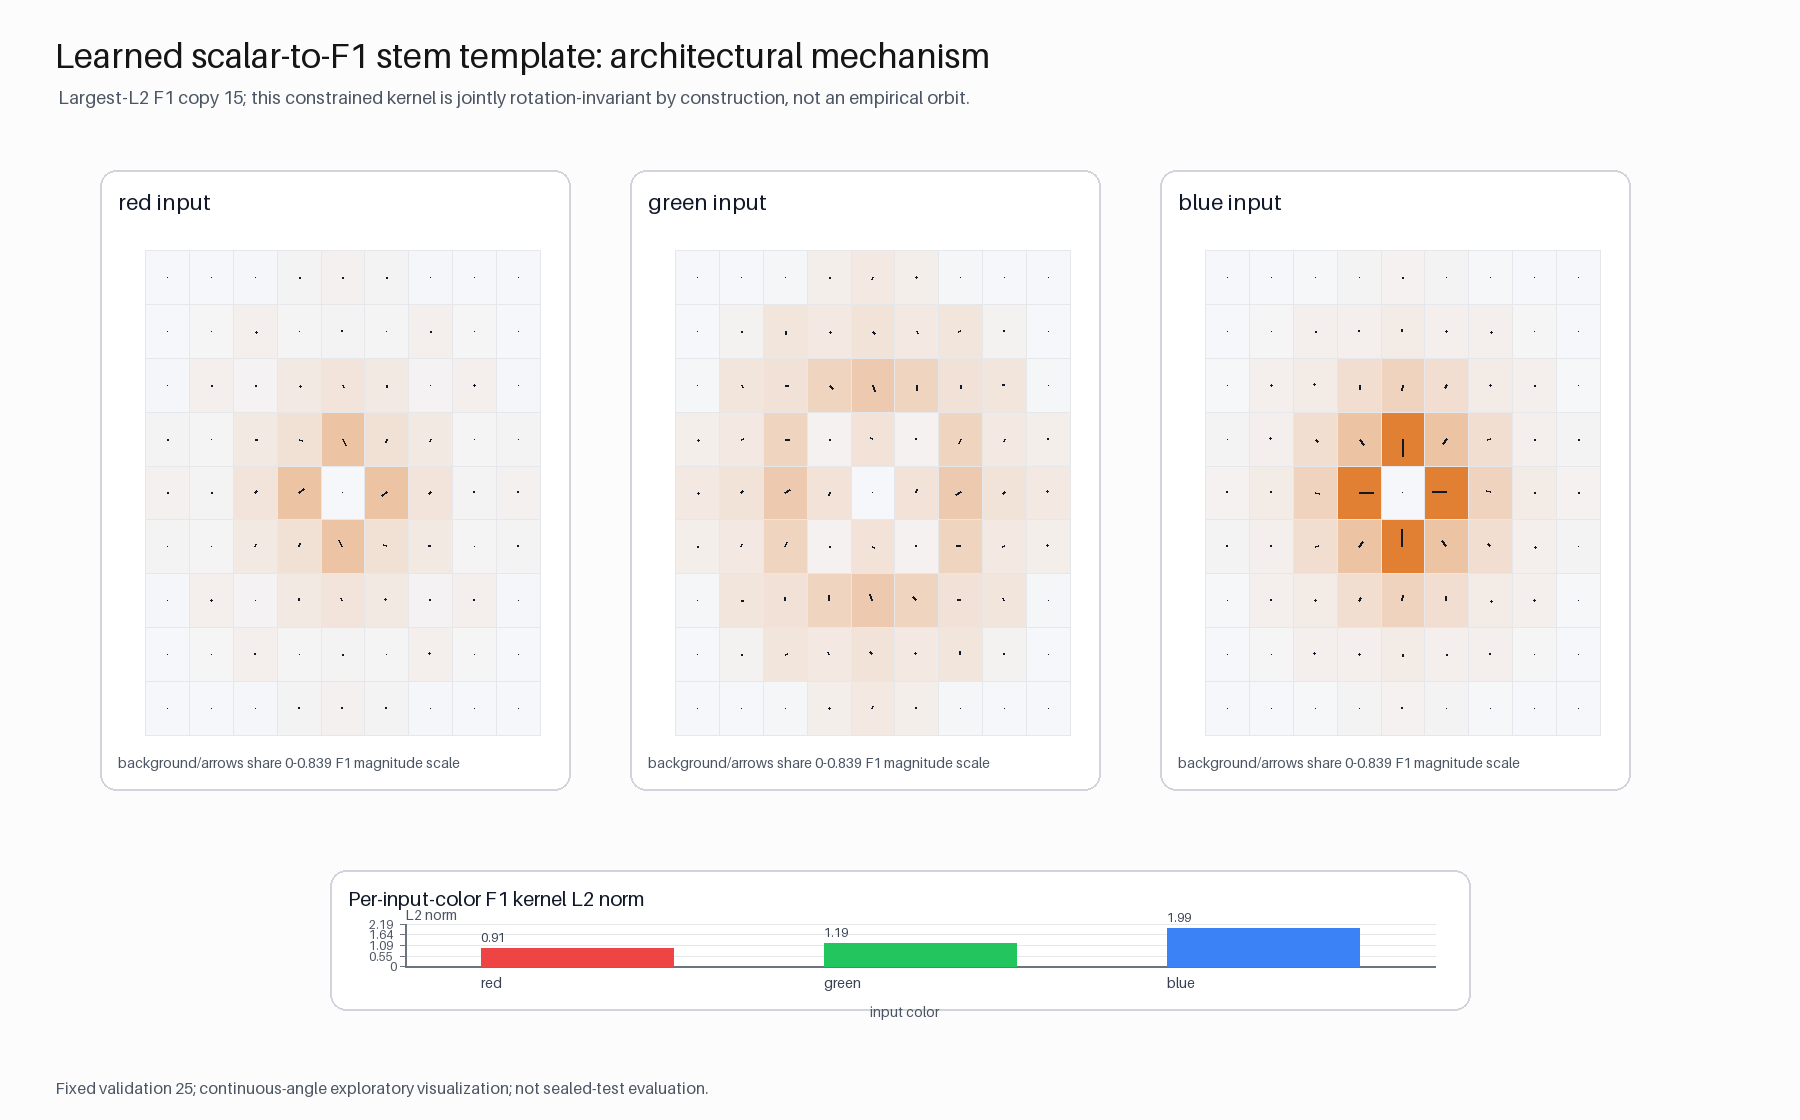
\includegraphics[width=\linewidth,trim=670 378 725 245,clip]
        {so2_stem_kernel_f1.png}
\end{minipage}\hfill
\begin{minipage}[t]{0.31\linewidth}
    \centering
    {\sffamily\small Canal azul\par}\smallskip
    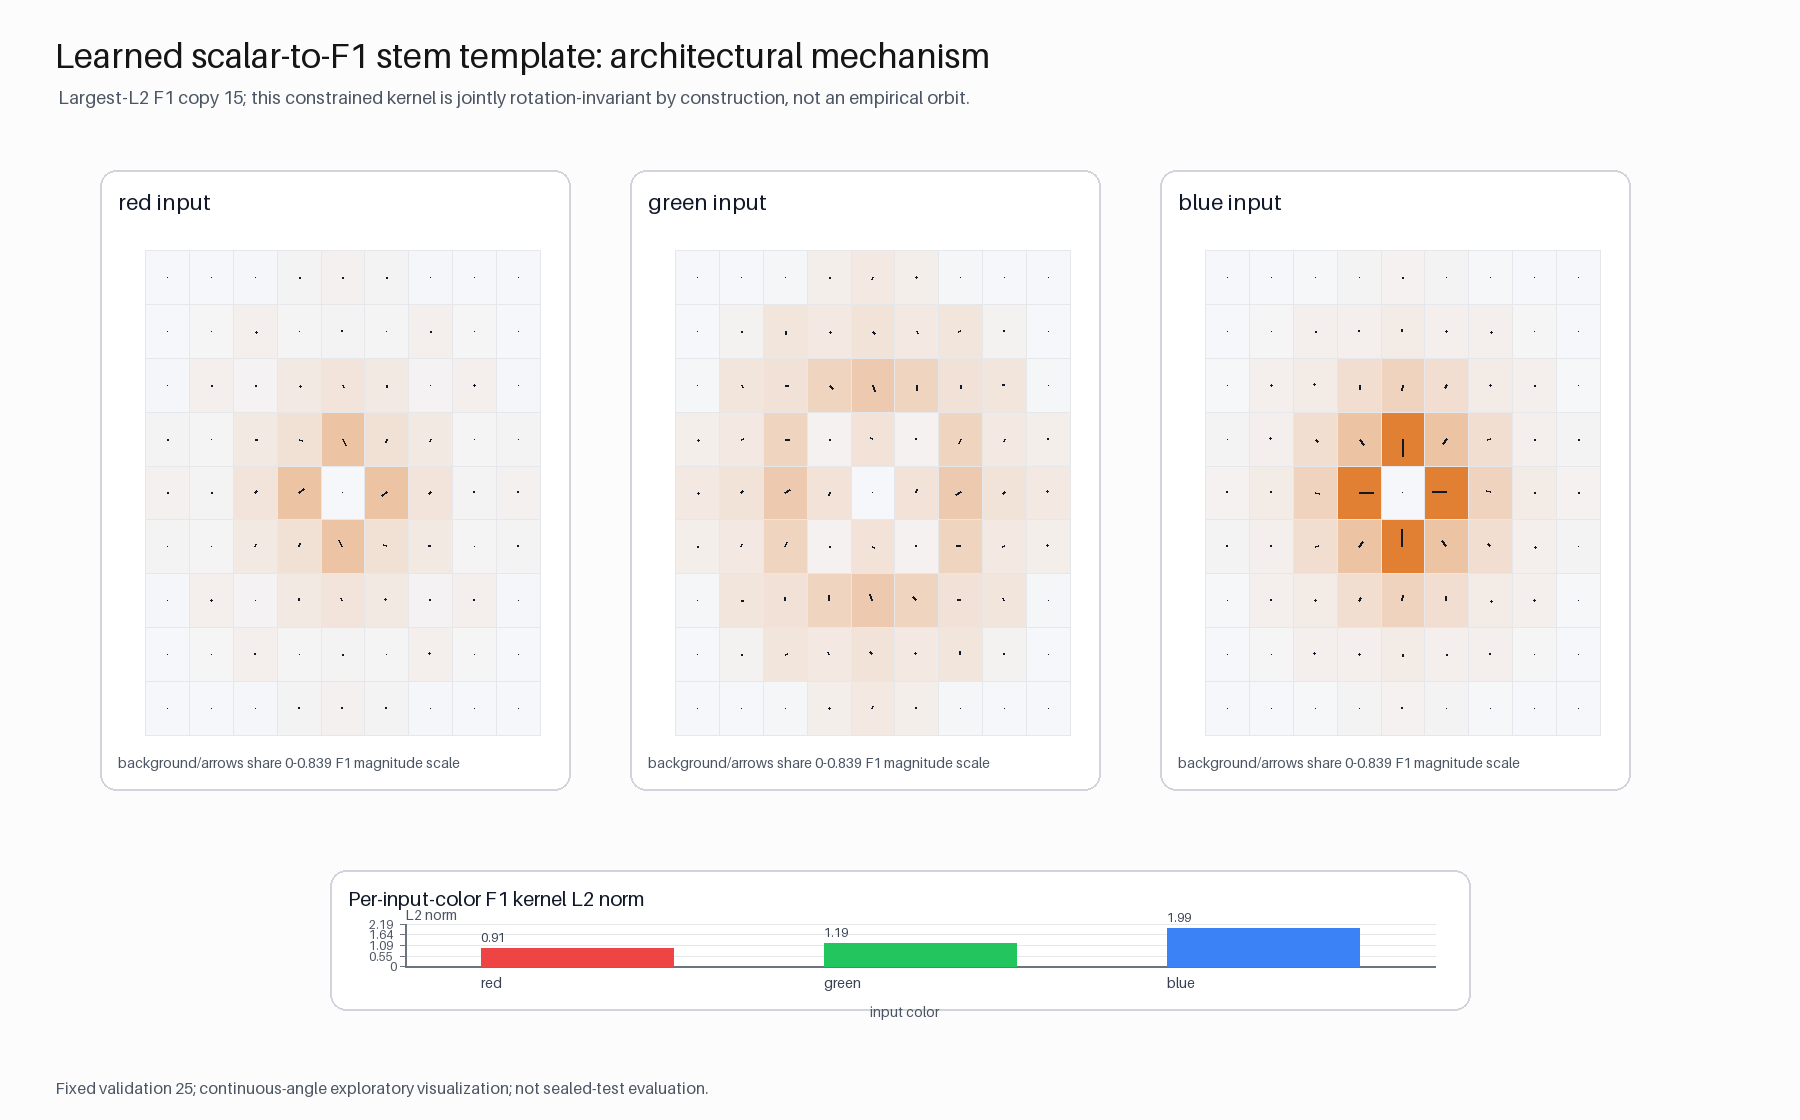
\includegraphics[width=\linewidth,trim=1200 378 195 245,clip]
        {so2_stem_kernel_f1.png}
\end{minipage}
\par\medskip
{\sffamily\small Escala de magnitud: 0--0,839\par}
\medskip
{\sffamily\small Norma $L_2$ por canal de entrada\par}
\smallskip
% Norms calculated from DATA.kernel.vectors in the accepted rotation-orbits.html.
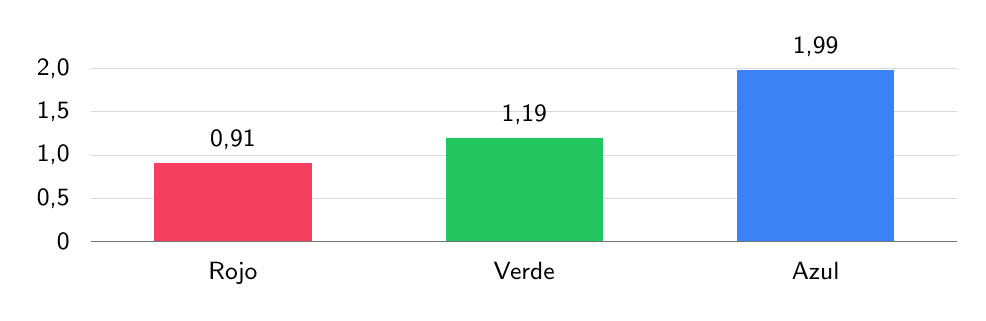
\begin{tikzpicture}[x=1cm,y=1.1cm,font=\sffamily\small]
    \foreach \y/\labeltext in {0/0,0.5/{0,5},1/{1,0},1.5/{1,5},2/{2,0}} {
        \draw[black!15] (0,\y) -- (11,\y);
        \node[anchor=east] at (-0.15,\y) {\labeltext};
    }
    \definecolor{kernelred}{HTML}{F43F5E}
    \definecolor{kernelgreen}{HTML}{22C55E}
    \definecolor{kernelblue}{HTML}{3B82F6}
    \foreach \x/\value/\displayvalue/\barcolor/\channel in {
        1.8/0.9145360512635107/{0,91}/kernelred/Rojo,
        5.5/1.194885652373353/{1,19}/kernelgreen/Verde,
        9.2/1.9877366483349737/{1,99}/kernelblue/Azul} {
        \fill[\barcolor] (\x-1.0,0) rectangle (\x+1.0,\value);
        \node[anchor=south] at (\x,\value+0.04) {\displayvalue};
        \node[anchor=north] at (\x,-0.12) {\channel};
    }
    \draw[black!55] (0,0) -- (11,0);
\end{tikzpicture}
